% ------------------------------------------------------------
\section{Calendar Week}
% ------------------------------------------------------------
% --------------------------------------------------- Slide --
\subsection{CW 31}
% ------------------------------------------------------------
\begin{frame}
  \frametitle{Review CW 31}
	\begin{itemize}
		\item Presence at MHH last Friday (06.08.21). "Remote Access" installed by IT. Tested by me both at MHH and at home. Everything working correctly so far! - \textcolor{green}{Done}.
		\item Added possibility of multi-steps for multiple lengths of the implant to created script. Objective: calculate and accumulate damage due to different lengths of the implant in a single run of the script. Further results obtained, see figure in next slide. \textcolor{green}{Done}.
	\end{itemize}
\end{frame}

\begin{frame}
  \frametitle{Review CW 31 - Model with Multi-Steps (compare with CW30 and 26)}
	\begin{figure}
		%\centering
		\subfigure{
		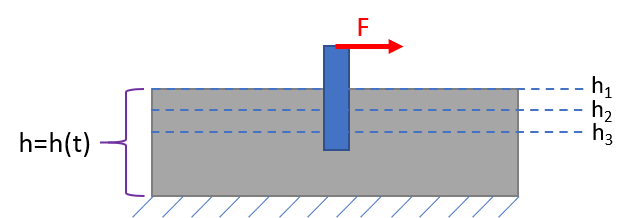
\includegraphics[width=0.45\textwidth]{pictures/CW26_1}
		}
		%\quad
		\subfigure{
		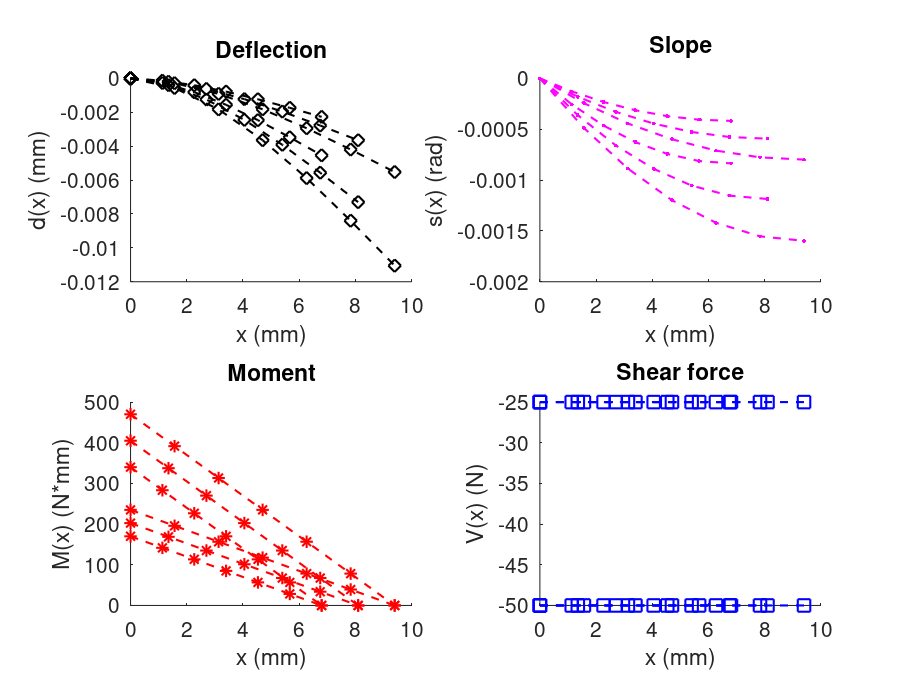
\includegraphics[width=0.45\textwidth]{pictures/CW31}
		}
	\end{figure}
\end{frame}

% ------------------------------------------------------------
% --------------------------------------------------- Slide --
\subsection{CW 32}
% ------------------------------------------------------------
% ------------------------------------------------------------
\begin{frame}
  \frametitle{Outlook CW 32}
	\begin{itemize}
		\item Perform more detailed FEA using Remote Access. Compare results from more detailed FEA with simplified analytical analysis.
	\end{itemize}
\end{frame}
% --------------------------------------------------- Slide --

